% Files using this must be two subfolders
% deep. Adjust the number of ../ for the
% depth of the file.
% Imports
\usepackage{fancyhdr}
\usepackage{geometry}
\usepackage{icomma}
\usepackage{amsmath}
\usepackage{multicol}
\usepackage{mathptmx}
\usepackage{anyfontsize}
\usepackage{t1enc}
\usepackage{tabto}
\usepackage{listings}
\usepackage{filecontents}
\usepackage{subcaption}
\usepackage{tikz}
\usepackage[parfill]{parskip}
\usepackage{graphicx}
\usepackage[]{mdframed}
\usepackage{amsmath}
\usepackage[makeroom]{cancel}
\usepackage{pgfplots}
\usepackage{pgfplotstable}
\usepackage{xfrac}
\usepackage{amssymb}
\usepackage{mathtools}
\pgfplotsset{compat=1.18}
\usetikzlibrary{patterns}
\usepgfplotslibrary{polar}
\usepgfplotslibrary{fillbetween}

\geometry{margin=2.5cm}

\newcommand{\name}{Kaleb Burris}
\newcommand{\classname}{MATH F253, Elizabeth S. Allman, University of Alaska Fairbanks}
\newcommand{\assignment}{FILL IN ASSIGNMENT NAME}

\pagestyle{fancy}

\fancyhead[L]{
    \name 
    \newline
    \classname
    \newline
    \assignment
}

\newcommand{\horizontal}{\noindent\rule{\hsize}{0.4pt}}

\setlength{\headheight}{42pt}
\setlength{\headsep}{0.25in}
\setlength{\columnsep}{0.35cm}
\setlength{\columnseprule}{1pt}

\usepackage[T1]{fontenc}
\usepackage{lmodern}

% Put class number, class name, and professor 
% name.
% Use only in case of emergency, this
% should be covered by the preamble.
% \renewcommand\classname{}

% Put the assignment name with \S if 
% necessary for the section and the question 
% numbers.
\renewcommand\assignment{Worksheet 15, Due February 27, 4:15pm}

\begin{document}
    % Templates
    \iffalse
    % Use these for equations.
    \begin{equation*}
        \begin{gathered}
            Equations go here.
        \end{gathered}
    \end{equation*}

    % Use this if a line of math is too long.
    \resizebox{\hsize}{!}{$Long equation goes here$}

    % Use these for multiple columns.
    \begin{multicol*}{# of columns}
        % Remove the * if you want the columns to be balanced.
    \end{multicol*}

    % Use this to add a horizontal line.
    \horizontal

    \fi

    % Begin homework here.
    %%%%%%%%%%%%%%%%%%%%%%

    \paragraph*{1.}\hbox{}

    \begin{enumerate}[label=(\alph*)]
        \item Find $p_{X}(x)$, the marginal pmf for $X$.
        
        \begin{mdframed}
            \begin{center}
                \begin{equation*}
                    \begin{array}{c | r}
                        X & P_{X}(x)  \\
                        \hline
                        1 & 0.13 + 0.53 + 0.24 = 0.90   \\
                        \hline
                        2 & 0.05 + 0.02 + 0.01 = 0.08   \\
                        \hline
                        3 & 0.02 + 0.00 + 0.00 = 0.02   \\
                        \hline
                          & 0.90 + 0.08 + 0.02 = 1.00
                    \end{array}
                \end{equation*}
            \end{center}
        \end{mdframed}

        \item Find $p_{Y}(y)$, the marginal pmf for $Y$.
        
        \begin{mdframed}
            \begin{equation*}
                \begin{array}{c | r}
                    Y & P_{Y}(y)  \\
                    \hline
                    0 & 0.13 + 0.05 + 0.02 = 0.20   \\
                    \hline
                    1 & 0.53 + 0.02 + 0.00 = 0.55   \\
                    \hline
                    2 & 0.25 + 0.01 + 0.00 = 0.26   \\
                    \hline
                      & 0.20 + 0.55 + 0.26 = 1.00
                \end{array}
            \end{equation*}
        \end{mdframed}

        \item Find $P(X = 1 \text { and } Y = 0)$.
        
        \begin{mdframed}
            \begin{equation*}
                P(X = 1 \text { and } Y = 0) = P\left(\begin{array}{l l} 1 & \text{hikes} \\ 0 & \text{trips to chicago} \end{array}\right) = \boxed{0.13}
            \end{equation*}
        \end{mdframed}

        \item Find $P(X = 0 \text { or } Y = 1)$.
        
        \begin{mdframed}
            \begin{align*}
                P(X = 1 \text { or } Y = 0) & = p_{X}(1) + p_{Y}(0) - P(X = 1, Y = 0)   \\
                                            & = 0.90 + 0.20 - 0.13 = \boxed{0.97}
            \end{align*}
        \end{mdframed}

        \item Find $P(X + Y = 2)$.
        
        \begin{mdframed}
            \begin{equation*}
                P(X + Y = 2) = 0.02 + 0.05 + 0.53 = \boxed{0.60}
            \end{equation*}
        \end{mdframed}
    \end{enumerate}

    \pagebreak

    \paragraph*{2.}
    Find the joint pdf of $X$ and $Y$ if $f(x,y)$, given below.

    \begin{equation*}
        f(x,y) = \begin{cases}
            \frac{1}{30}(3x^{2} + 2y) & \text{if } 1 \leq x \leq 2, 3 \leq y \leq 5 \\
            0 & \text{otherwise}
        \end{cases}
    \end{equation*}

    \begin{enumerate}[label=(\alph*)]
        \item Sketch the support of the joint distribution of $X$ and $Y$.
        
        \begin{mdframed}
            Bringing out the tikzplot for this one.

            \begin{tikzpicture}
                \begin{axis} [
                    xmin=1,xmax=2,
                    xlabel=x,ylabel=y,
                    ymin=3,ymax=5, axis equal
                ]

                    \addplot3[domain=1:2, domain y=3:5, samples=20, mesh]{(1/30)*(3*x^2 + 2*y)};
                    
                \end{axis}
            \end{tikzpicture}

            I have no idea but this is a neat plot.
        \end{mdframed}

        \item Find $P(3/2 \leq X \leq 2, 4 \leq Y \leq 5)$.
        
        \begin{mdframed}
            \begin{align*}
                P(3/2 \leq X \leq 2, 4 \leq Y \leq 5)   & = \int_{3/2}^{2}\left[\int_{4}^{5}\left(\frac{1}{30}(3x^{2} + 2y)\right)dy\right]dx   \\
                & = \int_{3/2}^{2}\left[\int_{4}^{5}\left(\frac{x^{2}}{30}\right)dy + \int_{4}^{5}\left(\frac{2y}{30}\right)dy\right]dx                    \\
                & = \int_{3/2}^{2}\left[\frac{x^{2}}{30} + 0.3\right]dx                                                                           \\
                & = \left[\frac{x^{3}}{90} + 0.3x \right]_{3/2}^{2} = \left(\frac{2^{3}}{90} + 0.6\right) - \left(\frac{(3/2)^{3}}{90} + 3/2(0.3)\right)      \\
                & = \left(\frac{8}{90} + 0.6\right) - \left(\frac{(27/8)}{90} + 0.45\right) = 0.6\overline{88} - 0.5075 = \boxed{0.1814}
            \end{align*}
        \end{mdframed}

        \pagebreak

        \item Find $f_{X}(x)$, the marginal distribution of $X$. Show that it integrates to 1.
        
        \begin{mdframed}
            \begin{align*}
                f_{X}(x)    & = \int_{-\infty}^{\infty}\left(\frac{1}{30}(3x^{2} + 2y)\right)dy                                 \\
                            & = \frac{1}{30}\int_{-\infty}^{\infty}(3x^2 + 2y)dy                                                \\
                            & \Rightarrow \frac{1}{30}\left[3x^{2}y + y^2\right]_{3}^{5}                                        \\
                            & = \frac{1}{30}\left[\left(15x^{2} + 25\right) - \left(9x^{2} + 9\right)\right]                    \\
                            & = \boxed{\frac{1}{30}\left[6x^2 + 16\right]}                                                      \\
                \int_{-\infty}^{\infty}f_{X}(x)dx & \Rightarrow \frac{1}{30}\int_{1}^{2}\left[6x^2 + 16\right]dx                \\
                            & = \frac{1}{30}\left[2x^{3} + 16x\right]_{1}^{2} = \frac{1}{30}\left[(16 + 32) - (2 + 16)\right]   \\
                            & = \frac{48 - 18}{30} = \frac{30}{30} = 1
            \end{align*}
        \end{mdframed}

        \item Find $f_{Y}(y)$, the marginal distribution of $Y$.
        
        \begin{mdframed}
            \begin{align*}
                f_{Y}(y)    & = \int_{-\infty}^{\infty}\left(\frac{1}{30}(3x^{2} + 2y)\right)dx                                 \\
                            & \Rightarrow \frac{1}{30}\int_{1}^{2}(3x^{2}+2y)dx                                                 \\
                            & = \frac{1}{30}\left[x^{3}+2yx\right]_{1}^{2} = \frac{1}{30}\left[(8 + 4y) - (1 + 2y)\right] = \boxed{\frac{2y + 7}{30}}
            \end{align*}
        \end{mdframed}
    \end{enumerate}

\end{document}